\subsection{Datenbank}
Das nachfolgende ERM-Diagramm zeigt die Struktur der Projektdatenbank auf.

\vspace{2mm}
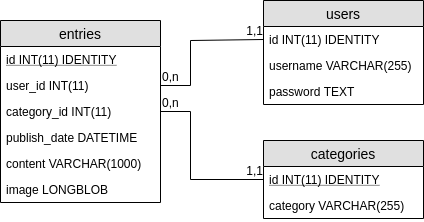
\includegraphics[scale=0.7]{database}
\vspace{2mm}

\noindent
Für den Zugriff wird zudem das Projekt \href{https://github.com/lincanbin/PHP-PDO-MySQL-Class}{lincanbin/PHP-PDO-MySQL-Class} verwendet. Es schnitt bei der Vorauswahl am besten ab, da es im Gegenzug zu kompletten Datenbank-Wrappern wir dem des Laravel-Frameworks nicht zu komplex ist, gegenüber der Programmierung mit Standard-PHP Funktionen aber doch eine enorme Zeitersparnis einbringt.

Bei einem Seitenaufruf wird so die Verbindung zur Datenbank einmalig von der Engine hergestellt und bleibt für alle Queries von Models offen.

Für Tests können somit auch langlebige Aktionen auf der Verbindungs-Instanz durchgeführt werden. Sämtliche Tests operieren auf der selben Verbindung, jeder Testfall wird aber in eine eigene Transaction verpackt, um sicherzustellen, dass Tests unabhängig voneinander ausgeführt werden.

\vspace{2mm}
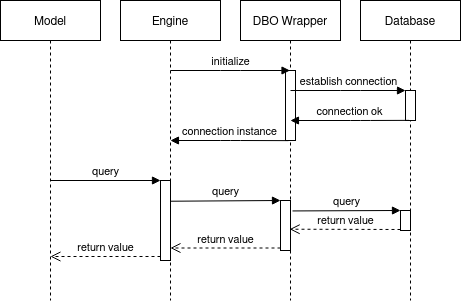
\includegraphics[scale=0.7]{dbengine}
\vspace{2mm}